\chapter{Introdução}
\label{ch:introducao}
\begin{resumocapitulo}
	Este capítulo apresenta uma visão geral do projeto de implantação de um e-commerce para a empresa Tech Inova Shop. Inicialmente, é contextualizada a necessidade da empresa de expandir sua presença no mercado digital diante do crescimento contínuo do comércio eletrônico e da demanda dos consumidores por uma experiência de compra online eficiente. Em seguida, são delineados os objetivos do projeto, que visam desenvolver uma plataforma de e-commerce robusta e escalável, com foco na melhoria da experiência do cliente e no aumento das vendas. O método utilizado para alcançar esses objetivos é descrito, incluindo análise de mercado, desenvolvimento de funcionalidades e estratégias de segurança e marketing. Por fim, são apresentadas as expectativas em relação aos resultados do projeto, destacando a importância de métricas como taxa de conversão e satisfação do cliente para avaliar o sucesso da implantação do e-commerce da Tech Inova Shop.
\end{resumocapitulo}

\section{Citações diretas e indiretas}
\label{sec:citacoes}
\subsection{Citação Direta}
\label{subsec:citacao_direta}
"O e-commerce revolucionou a forma como compramos e vendemos produtos e serviços, proporcionando uma experiência de compra mais conveniente, acessível e personalizada para os consumidores." (SILVA, 2020, p. 25).

\subsection{Citação Indireta}
\label{subsec:citacao_indireta}
De acordo com Silva (2020), o e-commerce trouxe consigo uma série de mudanças no cenário do varejo, impactando tanto o comportamento dos consumidores quanto as estratégias das empresas.
\section{Inclusão de Figura}
\label{sec:figura}
A figura 1.1 são diagramas do sistema
\begin{figure}[!ht]
	{\centering
		\caption{Diagrama DER.}
		
  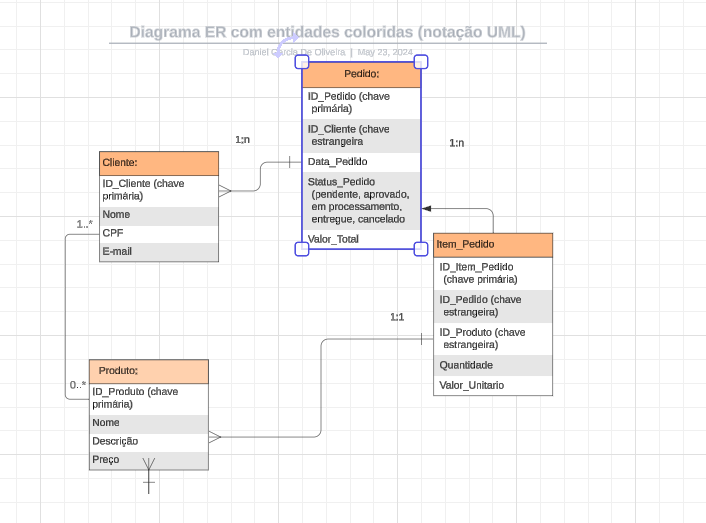
\includegraphics[width=0.9\textwidth]{figuras/dados.png}
  
  \caption{Modelo ER.}
  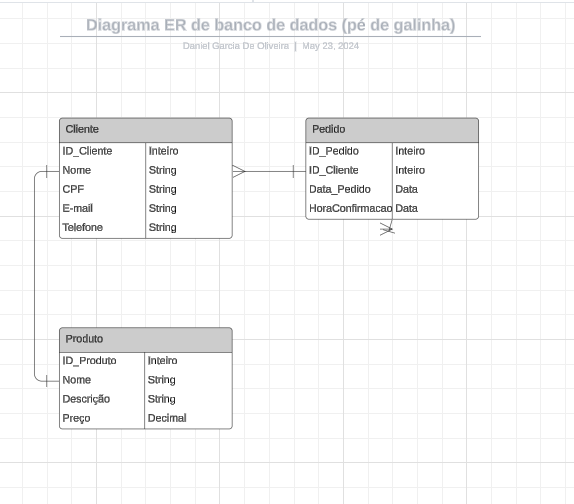
\includegraphics[width=0.9\textwidth]{figuras/dados1.png}
		\label{fig:identificador_da_figura}
		\fonte{Autor}
	}
\end{figure}

